% =====================================================================
%  DOSSIER DE DÉFINITION — BANC DE TEST CAN
%  Groupe 69 — ENSEA 2A — MANAGEMENT_PROJET_S7
%  Version 0.1 — 22/09/2026
%  Compilation : pdflatex (2 passes)
% =====================================================================
\documentclass[11pt,a4paper]{article}

\usepackage[utf8]{inputenc}
\usepackage[T1]{fontenc}
% lmodern non disponible ici
\usepackage[margin=2.2cm]{geometry}
\usepackage{graphicx}
\usepackage{booktabs}
\usepackage{array}
\usepackage{longtable}
\usepackage{xcolor}
\usepackage{siunitx}
\usepackage{tikz}
\usepackage[european,siunitx,RPvoltages]{circuitikz}
\usepackage{fancyhdr}
\usepackage{lastpage}
\usepackage{enumitem}
\usepackage{float}
\usepackage[hidelinks]{hyperref}

\usetikzlibrary{positioning,arrows.meta,calc,fit,backgrounds,shapes.geometric,decorations.pathmorphing}
\sisetup{locale=FR,per-mode=symbol}

% ---------- Métadonnées du document ----------
\newcommand{\docref}{G69-BANC-001}
\newcommand{\docversion}{v0.1}
\newcommand{\docdate}{22/09/2026}
\newcommand{\docstatus}{Brouillon — schémas uniquement}

% ---------- Couleurs ----------
\definecolor{canh}{RGB}{200,30,30}
\definecolor{canl}{RGB}{30,60,200}
\definecolor{nodefill}{RGB}{240,244,250}
\definecolor{mcufill}{RGB}{220,235,255}
\definecolor{trxfill}{RGB}{255,240,215}
\definecolor{toolfill}{RGB}{232,245,232}
\definecolor{grey}{RGB}{110,110,110}
\definecolor{oledfill}{RGB}{226,224,245}
\definecolor{todo}{RGB}{180,60,60}

% ---------- En-tête / pied de page ----------
\pagestyle{fancy}
\fancyhf{}
\lhead{\small Banc de test CAN — Dossier de définition}
\rhead{\small \docref{} — \docversion}
\lfoot{\small Groupe 69 — ENSEA 2A}
\rfoot{\small Page \thepage/\pageref{LastPage}}

\newcommand{\todo}[1]{\textcolor{todo}{\textit{[À rédiger : #1]}}}

% ---------- Styles TikZ ----------
\tikzset{
  node box/.style={draw, rounded corners=2pt, fill=nodefill, minimum width=2.35cm,
                   minimum height=3.0cm, align=center, font=\small, thick},
  oled/.style={draw, fill=oledfill, minimum width=2.0cm, minimum height=0.45cm,
               align=center, font=\scriptsize},
  mcu/.style={draw, fill=mcufill, minimum width=2.0cm, minimum height=0.5cm,
              align=center, font=\scriptsize},
  trx/.style={draw, fill=trxfill, minimum width=2.0cm, minimum height=0.5cm,
              align=center, font=\scriptsize},
  tool/.style={draw, rounded corners=2pt, fill=toolfill, minimum width=2.3cm,
               minimum height=1.0cm, align=center, font=\scriptsize, thick},
  lbl/.style={font=\scriptsize, text=grey, align=center},
  busH/.style={canh, very thick},
  busL/.style={canl, very thick},
  drop/.style={thick},
}

\begin{document}

% =====================================================================
%  PAGE DE TITRE
% =====================================================================
\begin{titlepage}
\centering
\vspace*{1.5cm}
{\large ENSEA — 2\textsuperscript{e} année — MANAGEMENT\_PROJET\_S7}\\[0.4cm]
{\large Projet 2A « Conception d'une Électronique Modulaire (Bus CAN) »}\\[2.5cm]

{\Huge\bfseries Dossier de définition}\\[0.5cm]
{\LARGE Banc de test CAN}\\[2cm]

\begin{tabular}{ll}
\toprule
Référence & \docref \\
Version & \docversion \\
Date & \docdate \\
Statut & \docstatus \\
\midrule
Groupe & 69 \\
Auteurs & Samuel GOMRI, Dylan KIATI, Hugo MATHOUX \\
Encadrants & Yves HECKEL, Julien SEIGNEURBIEUX \\
\midrule
Documents liés & ICD des groupes partenaires (documents distincts, cycles de vie propres) \\
\bottomrule
\end{tabular}

\vfill
\begin{minipage}{0.85\textwidth}
\small\itshape
Ce document décrit l'outil interne du groupe 69 servant à valider le standard CAN commun
et les ICD produits avec les groupes partenaires. Il est distinct des ICD : ceux-ci
décrivent l'interface convenue avec chaque projet, tandis que le présent dossier définit
le moyen de la vérifier. Le banc est générique et ne privilégie aucun projet : chaque
groupe partenaire est traité au même niveau, les besoins spécifiques étant couverts par
des variantes de configuration et non par une conception dédiée. Document vivant,
versionné à chaque évolution.
\end{minipage}
\vspace{1cm}
\end{titlepage}

\pagenumbering{roman}\tableofcontents
\newpage\pagenumbering{arabic}

% =====================================================================
\section{Objet et périmètre}
% =====================================================================
\todo{rédaction complète du périmètre}

Le banc de test doit permettre de démontrer les six fonctions suivantes, qui structurent
le protocole de validation (\S\ref{sec:protocole}) :
\begin{enumerate}[nosep]
  \item Validation de la couche physique (niveaux différentiels, terminaisons, débit \SI{500}{kbit/s}) ;
  \item Démonstration de l'arbitrage entre au moins trois nœuds émetteurs simultanés ;
  \item Validation de l'encodage des messages définis dans l'ICD ;
  \item Tests de robustesse par injection de fautes ;
  \item Démonstration pédagogique à destination de l'ensemble des groupes partenaires, sans distinction de projet ;
  \item Validation de l'isolation galvanique, pour toute intégration à proximité d'électronique de puissance.
\end{enumerate}

% =====================================================================
\section{Architecture de principe}
% =====================================================================

Le banc est constitué d'un noyau fonctionnel (nœuds + couche physique + câblage) sur
lequel se greffent des équipements de mesure et de visualisation branchés en dérivation.

\subsection{Schéma bloc}

\begin{figure}[h]
\centering
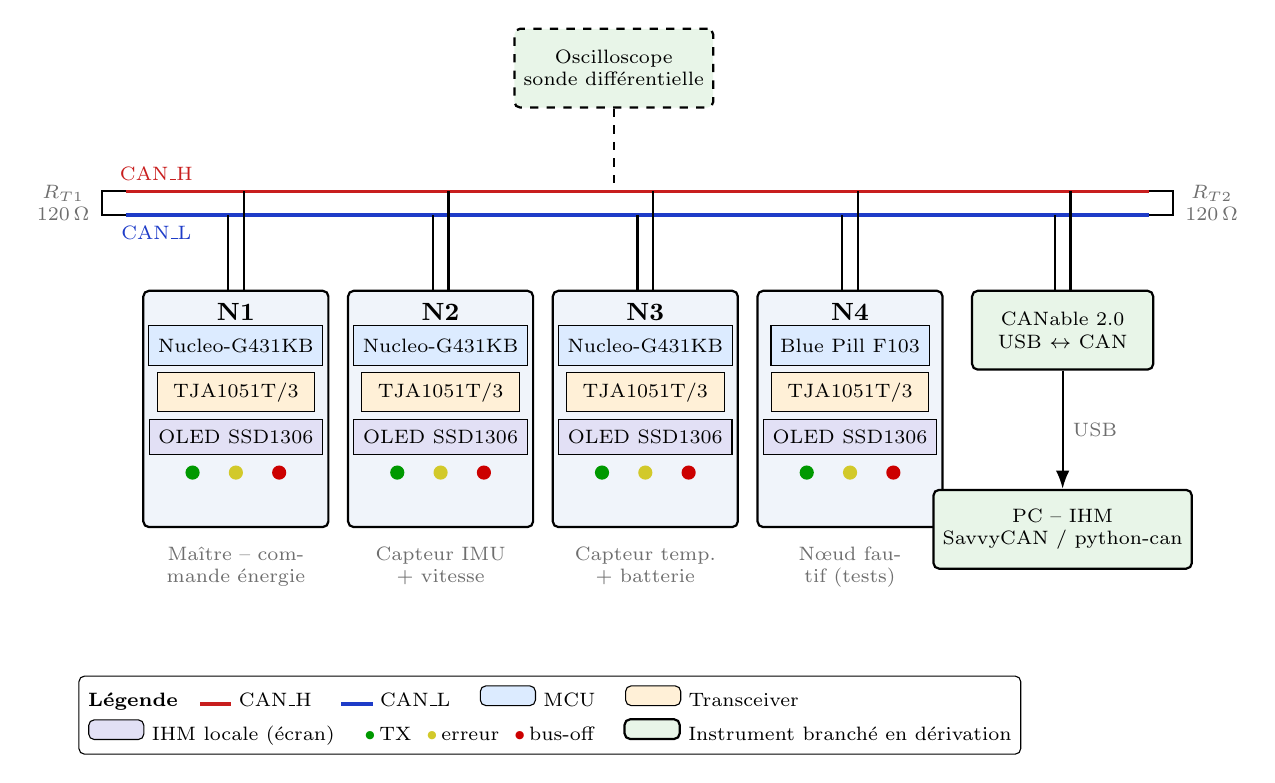
\begin{tikzpicture}[x=1cm,y=1cm]

% ---- Bus ----
\coordinate (BL) at (0,0);
\coordinate (BR) at (13.0,0);
\draw[busH] (BL) ++(0,0.15) -- ++(13.0,0) node[pos=0.03, above, lbl, canh] {CAN\_H};
\draw[busL] (BL) ++(0,-0.15) -- ++(13.0,0) node[pos=0.03, below, lbl, canl] {CAN\_L};

% ---- Terminaisons ----
\draw[thick] (0,0.15) -- (-0.3,0.15) -- (-0.3,-0.15) -- (0,-0.15);
\node[lbl, left=1pt] at (-0.3,0) {$R_{T1}$\\\SI{120}{\ohm}};
\draw[thick] (13.0,0.15) -- (13.3,0.15) -- (13.3,-0.15) -- (13.0,-0.15);
\node[lbl, right=1pt] at (13.3,0) {$R_{T2}$\\\SI{120}{\ohm}};

% ---- Nœuds ----
\foreach \x/\name/\role/\mcu in {
   1.4/N1/Maître -- commande énergie/Nucleo-G431KB,
   4.0/N2/Capteur IMU + vitesse/Nucleo-G431KB,
   6.6/N3/Capteur temp. + batterie/Nucleo-G431KB,
   9.2/N4/Nœud fautif (tests)/Blue Pill F103}
{
  \node[node box, anchor=north] (\name) at (\x,-1.1) {};
  \node[font=\small\bfseries, anchor=north] at ($(\name.north)+(0,-0.05)$) {\name};
  \node[mcu, anchor=north] (\name m) at ($(\name.north)+(0,-0.45)$) {\mcu};
  \node[trx, anchor=north] (\name t) at ($(\name m.south)+(0,-0.08)$) {TJA1051T/3};
  \node[oled, anchor=north] (\name o) at ($(\name t.south)+(0,-0.08)$) {OLED SSD1306};
  % LEDs d'etat
  \fill[green!60!black] ($(\name o.south)+(-0.55,-0.22)$) circle (0.09);
  \fill[yellow!80!black] ($(\name o.south)+(0,-0.22)$) circle (0.09);
  \fill[red!80!black]   ($(\name o.south)+(0.55,-0.22)$) circle (0.09);
  \node[lbl, anchor=north, text width=2.3cm, align=center] at ($(\name.south)+(0,-0.12)$) {\role};
  % dérivation
  \draw[drop] (\x-0.1,-1.1) -- (\x-0.1,-0.15);
  \draw[drop] (\x+0.1,-1.1) -- (\x+0.1,0.15);
}

% ---- Sniffer + IHM ----
\node[tool, anchor=north] (CAB) at (11.9,-1.1) {CANable 2.0\\ \scriptsize USB $\leftrightarrow$ CAN};
\draw[drop] (11.8,-1.1) -- (11.8,-0.15);
\draw[drop] (12.0,-1.1) -- (12.0,0.15);
\node[tool, below=1.5cm of CAB] (PC) {PC -- IHM\\ \scriptsize SavvyCAN / python-can};
\draw[-{Latex}, thick] (CAB) -- (PC) node[midway, right, lbl] {USB};

% ---- Oscilloscope ----
\node[tool, dashed, anchor=south] (OSC) at (6.2,1.2) {Oscilloscope\\ \scriptsize sonde différentielle};
\draw[dashed, thick] (OSC.south) -- (6.2,0.15);

% ---- Légende ----
\node[draw, rounded corners=2pt, font=\scriptsize, align=left, anchor=north west] at (-0.6,-6.0) {
  \textbf{Légende}\quad
  \textcolor{canh}{\rule{0.4cm}{1.5pt}} CAN\_H \quad
  \textcolor{canl}{\rule{0.4cm}{1.5pt}} CAN\_L \quad
  \tikz\node[mcu, minimum width=0.7cm, minimum height=0.25cm]{}; MCU \quad
  \tikz\node[trx, minimum width=0.7cm, minimum height=0.25cm]{}; Transceiver \\[2pt]
  \tikz\node[oled, minimum width=0.7cm, minimum height=0.25cm]{}; IHM locale (écran) \quad
  \textcolor{green!60!black}{$\bullet$}\,TX \ \textcolor{yellow!80!black}{$\bullet$}\,erreur \ \textcolor{red!80!black}{$\bullet$}\,bus-off \quad
  \tikz\node[tool, minimum width=0.7cm, minimum height=0.25cm]{}; Instrument branché en dérivation
};
\end{tikzpicture}
\caption{Architecture de principe du banc : quatre nœuds sur un bus terminé aux deux extrémités.
Chaque nœud porte sa propre IHM locale (écran et LEDs) ; instrumentation et IHM PC sont en dérivation.}
\label{fig:archi}
\end{figure}

\subsection{Principe de lecture}
\begin{itemize}[nosep]
  \item Chaque nœud est composé d'un microcontrôleur (contrôleur CAN intégré) et d'un transceiver
        qui réalise l'interface électrique avec le bus.
  \item Le bus est une paire torsadée terminée par \SI{120}{\ohm} à \emph{chacune} de ses deux
        extrémités, et uniquement là.
  \item Le sniffer CANable est un nœud passif supplémentaire : il acquitte les trames mais n'en émet
        pas hors phases d'injection volontaire.
  \item L'oscilloscope observe le signal différentiel sans charger le bus.
\end{itemize}

\subsection{Choix des composants structurants}
\begin{description}[nosep]
  \item[Microcontrôleur] STM32 (Nucleo-G431KB), aligné sur la cible des groupes partenaires.
        Le périphérique FDCAN est configuré en mode \emph{Classic} (CAN~2.0A, identifiants 11 bits,
        \SI{500}{kbit/s}) ; la capacité CAN~FD reste disponible sans changement matériel.
  \item[Transceiver] TJA1051T/3 : alimentation $V_{CC}=\SI{5}{V}$ pour des niveaux différentiels
        conformes ISO~11898-2, broche $V_{IO}=\SI{3.3}{V}$ pour une interface logique directe avec
        le STM32 sans adaptation de niveau. Ce choix répond au point soulevé par l'encadrement sur
        la tension d'alimentation.
\end{description}

% =====================================================================
\section{Nomenclature}
% =====================================================================
\todo{BOM détaillée par lot avec références fournisseur et coûts}

% =====================================================================
\section{Schémas électriques}
% =====================================================================

% ---------------------------------------------------------------------
\subsection{Schéma type d'un nœud (Nucleo-G431KB + TJA1051T/3)}
\label{sec:noeud}
% ---------------------------------------------------------------------

Le schéma ci-dessous est identique pour N1, N2 et N3. Le nœud N4 (Blue Pill STM32F103)
suit le même principe avec les broches PA11/PA12 du bxCAN.

\begin{figure}[h]
\centering
\begin{circuitikz}[american, scale=0.9, transform shape]

% ---------- Nucleo (bloc) ----------
\node[draw, thick, fill=mcufill, minimum width=3.6cm, minimum height=5.2cm, anchor=south west]
  (NUC) at (0,-0.4) {};
\node[font=\small\bfseries, anchor=north] at ($(NUC.north)+(0,-0.15)$) {Nucleo-G431KB};
\node[font=\scriptsize, anchor=north] at ($(NUC.north)+(0,-0.55)$) {STM32G431KB};

% broches c\^ot\'e droit du Nucleo (x = 3.6)
\coordinate (pTX)  at (3.6,3.6);
\coordinate (pRX)  at (3.6,2.8);
\coordinate (p5V)  at (3.6,2.0);
\coordinate (pGND) at (3.6,1.2);
\coordinate (p3V3) at (3.6,0.4);
\foreach \p/\t in {pTX/PA12 -- FDCAN1\_TX, pRX/PA11 -- FDCAN1\_RX, p5V/5V, pGND/GND, p3V3/3V3}
  \node[font=\scriptsize, anchor=east] at ($(\p)+(-0.1,0)$) {\t};
\foreach \p in {pTX,pRX,p5V,pGND,p3V3} \fill (\p) circle (1.2pt);

% ---------- TJA1051T/3 (bloc) ----------
\node[draw, thick, fill=trxfill, minimum width=3.2cm, minimum height=5.2cm, anchor=south west]
  (TRX) at (8.6,-0.4) {};
\node[font=\small\bfseries, anchor=north] at ($(TRX.north)+(0,-0.15)$) {TJA1051T/3};
\node[font=\scriptsize, anchor=north] at ($(TRX.north)+(0,-0.55)$) {transceiver CAN -- SO8};

% broches gauche (x = 8.6), ordre fonctionnel
\coordinate (tTXD) at (8.6,3.6);
\coordinate (tRXD) at (8.6,2.8);
\coordinate (tVCC) at (8.6,2.0);
\coordinate (tGND) at (8.6,1.2);
\coordinate (tVIO) at (8.6,0.4);
\foreach \p/\t in {tTXD/TXD (1), tRXD/RXD (4), tVCC/$V_{CC}$ (3), tGND/GND (2), tVIO/$V_{IO}$ (5)}
  \node[font=\scriptsize, anchor=west] at ($(\p)+(0.1,0)$) {\t};
\foreach \p in {tTXD,tRXD,tVCC,tGND,tVIO} \fill (\p) circle (1.2pt);
% broches droite (x = 11.8)
\coordinate (tS)    at (11.8,3.6);
\coordinate (tCANH) at (11.8,2.4);
\coordinate (tCANL) at (11.8,1.6);
\foreach \p/\t in {tS/(8) S, tCANH/(7) CANH, tCANL/(6) CANL}
  \node[font=\scriptsize, anchor=east] at ($(\p)+(-0.1,0)$) {\t};
\foreach \p in {tS,tCANH,tCANL} \fill (\p) circle (1.2pt);

% ---------- Liaisons Nucleo <-> transceiver (lignes droites parall\`eles) ----------
\draw (pTX)  -- (tTXD) node[pos=0.5, above, font=\scriptsize] {TXD -- \SI{3.3}{V}};
\draw (pRX)  -- (tRXD) node[pos=0.5, above, font=\scriptsize] {RXD -- niveau $V_{IO}$};
\draw (p5V)  -- (tVCC) node[pos=0.13, above, font=\scriptsize] {+5V};
\draw (pGND) -- (tGND) node[pos=0.13, above, font=\scriptsize] {GND};
\draw (p3V3) -- (tVIO) node[pos=0.13, above, font=\scriptsize] {+3V3};

% ---------- D\'ecouplage (entre lignes adjacentes, sans croisement) ----------
\draw (6.0,2.0) to[C, l_=$C_1$] (6.0,1.2);
\fill (6.0,2.0) circle (1.2pt); \fill (6.0,1.2) circle (1.2pt);
\draw (7.2,1.2) to[C, l_=$C_2$] (7.2,0.4);
\fill (7.2,1.2) circle (1.2pt); \fill (7.2,0.4) circle (1.2pt);
% masse de r\'ef\'erence
\draw (5.0,1.2) -- (5.0,0.85) node[ground]{};
\fill (5.0,1.2) circle (1.2pt);

% ---------- Broche S : mode normal ----------
\draw (tS) -- ++(1.0,0) -- ++(0,-0.4) node[ground]{};
\node[font=\scriptsize, anchor=south west] at ($(tS)+(0.15,0.05)$) {mode normal};

% ---------- Sortie bus + connecteur DB9 ----------
\draw[canh, thick] (tCANH) -- ++(2.8,0) coordinate (jH);
\draw[canl, thick] (tCANL) -- ++(2.8,0) coordinate (jL);
\coordinate (jG) at ($(jL)+(0,-1.0)$);
\draw (jG) ++(-1.6,0) node[ground]{} -- (jG);
\node[draw, thick, minimum width=1.7cm, minimum height=2.6cm, anchor=west, fill=white]
  (J) at ($(jH)+(0,-0.8)$) {};
\node[font=\scriptsize\bfseries, anchor=south] at (J.north) {J1 -- DB9};
\node[font=\scriptsize, anchor=west] at ($(jH)+(0.15,0)$) {7 \ CAN\_H};
\node[font=\scriptsize, anchor=west] at ($(jL)+(0.15,0)$) {2 \ CAN\_L};
\node[font=\scriptsize, anchor=west] at ($(jG)+(0.15,0)$) {3 \ GND};
\fill (jH) circle (1.2pt); \fill (jL) circle (1.2pt); \fill (jG) circle (1.2pt);

\end{circuitikz}

\caption{Schéma électrique d'un nœud : le STM32 dialogue en \SI{3.3}{V} avec le transceiver
via $V_{IO}$ ; le transceiver est alimenté en \SI{5}{V} côté bus. Broche S à la masse
pour le mode normal (haute vitesse).}
\label{fig:noeud}
\end{figure}

\begin{table}[H]
\centering\small
\begin{tabular}{llll}
\toprule
\textbf{Nucleo-G431KB} & \textbf{TJA1051T/3} & \textbf{Fonction} & \textbf{Remarque} \\
\midrule
PA12 (FDCAN1\_TX) & 1 -- TXD & Données MCU $\rightarrow$ bus & niveau \SI{3.3}{V} \\
PA11 (FDCAN1\_RX) & 4 -- RXD & Données bus $\rightarrow$ MCU & niveau $V_{IO}$ \\
3V3 & 5 -- $V_{IO}$ & Référence logique & fixe le seuil TXD/RXD \\
5V & 3 -- $V_{CC}$ & Alimentation étage bus & \SI{4.5}{V} à \SI{5.5}{V} \\
GND & 2 -- GND & Masse commune & reliée au GND du bus (DB9-3) \\
-- & 8 -- S & Sélection de mode & à GND = normal ; à $V_{IO}$ = silencieux \\
-- & 7 -- CANH & Bus & DB9 broche 7 \\
-- & 6 -- CANL & Bus & DB9 broche 2 \\
\bottomrule
\end{tabular}
\caption{Correspondance des broches pour un nœud. Les repères Arduino Nano des broches PA11/PA12
sur la Nucleo-32 sont à confirmer sur le manuel UM2397 avant câblage.}
\end{table}

\paragraph{Points de conception.}
\begin{itemize}[nosep]
  \item La broche \textbf{S} permet, si elle est reliée à une GPIO au lieu de GND, de placer le nœud
        en mode \emph{silencieux} (écoute seule) par logiciel : utile pour le protocole de validation
        (nœud témoin) sans recâblage.
  \item Les condensateurs de découplage $C_1$ (sur $V_{CC}$) et $C_2$ (sur $V_{IO}$) valent \SI{100}{nF} chacun et sont placés au plus près des broches du transceiver.
  \item Le \SI{5}{V} peut être pris sur la broche 5V du Nucleo (alimenté par USB) ou sur le rail
        \SI{5}{V} du banc (\S\ref{sec:alim}). Ne pas connecter les deux sources simultanément.
\end{itemize}

% ---------------------------------------------------------------------
\subsection{Schéma du bus complet}
\label{sec:bus}
% ---------------------------------------------------------------------

\begin{figure}[h]
\centering
\begin{circuitikz}[american, scale=0.9, transform shape]

% Bus
\draw[canh, very thick] (0,1) -- (15,1);
\draw[canl, very thick] (0,0) -- (15,0);
\node[canh, font=\scriptsize, anchor=south] at (12.2,1.12) {CAN\_H};
\node[canl, font=\scriptsize, anchor=north] at (12.2,-0.12) {CAN\_L};

% Terminaisons
\draw (0,1) to[R, l_=$R_{T1}$ \SI{120}{\ohm}] (0,0);
\draw (15,1) to[R, l=$R_{T2}$ \SI{120}{\ohm}] (15,0);

% Dérivations (stubs)
\foreach \x/\n in {2/J1, 5/J2, 8/J3, 11/J4, 13.5/J5}
{
  \draw[canh, thick] (\x-0.15,1) -- (\x-0.15,-0.8);
  \draw[canl, thick] (\x+0.15,0) -- (\x+0.15,-0.8);
  \node[draw, thick, fill=white, minimum width=1.0cm, minimum height=0.5cm, anchor=north,
        font=\scriptsize] at (\x,-0.8) {\n{} DB9};
}
\foreach \x/\t in {2/N1, 5/N2, 8/N3, 11/N4, 13.5/CANable}
  \node[font=\scriptsize\bfseries, anchor=north] at (\x,-1.45) {\t};

% Cotes
\draw[<->, grey] (0,1.6) -- (15,1.6) node[midway, above, font=\scriptsize, text=grey]
  {longueur totale $L \le \SI{5}{m}$ (banc) — $L_{max}=\SI{100}{m}$ à \SI{500}{kbit/s}};
\node[font=\scriptsize, text=grey, anchor=west] at (15.3,-0.5) {stubs $\le \SI{0.3}{m}$};

% Blindage / masse
\draw[dashed, grey] (0,-3.1) -- (15,-3.1);
\node[font=\scriptsize, text=grey, anchor=south west] at (0,-3.1) {Blindage / GND de référence — relié à la masse en un seul point};
\draw (7.5,-3.1) node[ground]{};

\end{circuitikz}
\caption{Topologie du bus : ligne principale terminée aux deux extrémités, cinq points de
raccordement en dérivation courte. Le CANable occupe le dernier connecteur.}
\label{fig:bus}
\end{figure}

\paragraph{Brochage DB9 (CiA 303-1).} Tous les connecteurs du banc utilisent le même brochage
afin qu'un nœud puisse être branché sur n'importe quel point sans risque d'erreur.

\begin{table}[H]
\centering\small
\begin{tabular}{clc}
\toprule
\textbf{Broche DB9} & \textbf{Signal} & \textbf{Couleur préconisée} \\
\midrule
2 & CAN\_L & bleu \\
3 & GND (référence) & noir \\
7 & CAN\_H & rouge (ou blanc) \\
9 & +5V (optionnel, alimentation d'un nœud) & rouge \\
1, 4, 5, 6, 8 & non connectés & -- \\
\bottomrule
\end{tabular}
\caption{Brochage des connecteurs J1 à J5.}
\end{table}

\paragraph{Règles de topologie.}
\begin{itemize}[nosep]
  \item Deux terminaisons exactement, aux deux extrémités physiques de la ligne.
  \item Dérivations (stubs) les plus courtes possible ; aucun nœud « en bout de stub long ».
  \item Le blindage du câble est relié à la masse en un seul point (éviter les boucles de masse) ;
        ce point est à reprendre au cas par cas lors de chaque intégration (isolation galvanique).
\end{itemize}

% ---------------------------------------------------------------------
\subsection{Distribution d'alimentation}
\label{sec:alim}
% ---------------------------------------------------------------------

\begin{figure}[h]
\centering
\begin{circuitikz}[american, scale=0.9, transform shape]

% ---------- Source ----------
\node[draw, thick, minimum width=2.4cm, minimum height=1.5cm, align=center, font=\small]
  (PSU) at (0,0) {Alim. labo\\ \SI{12}{V} / \SI{3}{A}};

% ---------- Convertisseur ----------
\node[draw, thick, fill=toolfill, minimum width=2.6cm, minimum height=1.5cm, align=center,
      font=\small] (DC) at (4.4,0) {DC/DC LM2596\\ \scriptsize $\SI{12}{V}\to\SI{5}{V}$};

\draw (PSU.east) ++(0,0.35) -- ($(DC.west)+(0,0.35)$)
  node[midway, above, font=\scriptsize] {+12V};
\draw (PSU.east) ++(0,-0.35) -- ($(DC.west)+(0,-0.35)$)
  node[midway, below, font=\scriptsize] {GND};

% ---------- Rails ----------
\coordinate (r5a) at (6.0,0.35);
\coordinate (r5b) at (15.4,0.35);
\coordinate (rga) at (6.0,-0.95);
\coordinate (rgb) at (15.4,-0.95);
\draw[very thick] (r5a) -- (r5b);
\draw[very thick] (rga) -- (rgb);
\node[font=\scriptsize\bfseries, anchor=south west] at ($(r5a)+(0.05,0.12)$) {Rail +5V};
\node[font=\scriptsize\bfseries, anchor=north west] at ($(rga)+(0.05,-0.12)$) {Rail GND};
\draw (DC.east) ++(0,-0.35) -- (6.0,-0.35) -- (rga);
\draw (DC.east) ++(0,0.35) -- (r5a);
\draw (7.5,-0.95) -- (7.5,-1.55) node[ground]{};
\fill (7.5,-0.95) circle (1.4pt);

% ---------- Condensateur de rail ----------
\draw (6.8,0.35) to[C, l=\SI{100}{\micro F}] (6.8,-0.95);
\fill (6.8,0.35) circle (1.4pt); \fill (6.8,-0.95) circle (1.4pt);

% ---------- Consommateurs ----------
\foreach \x/\nom/\det in {
   9.4/{N1 -- N3}/{Nucleo VIN (5V)\\ + TJA $V_{CC}$},
  11.9/{N4}/{Blue Pill 5V\\ + TJA $V_{CC}$},
  14.4/{Option}/{DB9 broche 9\\ (alim. distante)}}
{
  % descente +5V avec saut au-dessus du rail GND
  \draw (\x-0.35,0.35) -- (\x-0.35,-0.77);
  \draw (\x-0.35,-0.77) arc (180:0:0.18);
  \draw (\x+0.01,-0.77) -- (\x+0.01,-1.7);
  \draw (\x-0.35,-1.13) -- (\x-0.35,-1.7) -- (\x+0.01,-1.7);
  \draw (\x+0.35,-0.95) -- (\x+0.35,-1.7);
  \fill (\x-0.35,0.35) circle (1.4pt); \fill (\x+0.35,-0.95) circle (1.4pt);
  \node[draw, thick, fill=nodefill, minimum width=2.1cm, minimum height=1.1cm, align=center,
        font=\scriptsize, anchor=north] at (\x,-1.7) {\textbf{\nom}\\ \det};
}

% ---------- R\'egulateur interne -> 3V3 ----------
\node[draw, dashed, fill=mcufill, minimum width=2.1cm, minimum height=0.8cm, align=center,
      font=\scriptsize, anchor=north] (LDO) at (9.4,-3.4)
      {LDO Nucleo\\ $\SI{5}{V}\to\SI{3.3}{V}$};
\draw[-{Latex}] (9.4,-2.8) -- (LDO.north);
\node[font=\scriptsize, anchor=north, align=center] at ($(LDO.south)+(0,-0.1)$)
  {$\rightarrow V_{IO}$ du transceiver};

\end{circuitikz}
\caption{Distribution d'alimentation : un rail \SI{5}{V} unique issu d'un convertisseur DC/DC,
le \SI{3.3}{V} de chaque nœud est produit localement par le régulateur de sa carte.}
\label{fig:alim}
\end{figure}

\paragraph{Bilan de puissance (ordre de grandeur).} Les valeurs ci-dessous sont des estimations à confirmer par la mesure lors de la recette du banc.

\begin{table}[H]
\centering\small
\begin{tabular}{lccc}
\toprule
\textbf{Consommateur} & \textbf{Courant typ.} & \textbf{Qté} & \textbf{Total} \\
\midrule
Nucleo-G431KB (\SI{5}{V}) & \SI{60}{mA} & 3 & \SI{180}{mA} \\
Blue Pill F103 (\SI{5}{V}) & \SI{40}{mA} & 1 & \SI{40}{mA} \\
TJA1051T/3 en émission & \SI{50}{mA} & 4 & \SI{200}{mA} \\
Capteurs (IMU, Hall, DS18B20) & \SI{20}{mA} & -- & \SI{40}{mA} \\
\midrule
\textbf{Total estimé} & & & \textbf{$\approx$ \SI{0.5}{A}} \\
\bottomrule
\end{tabular}
\caption{Bilan de puissance : un convertisseur \SI{2}{A} offre une marge confortable.}
\end{table}

\paragraph{Règles.}
\begin{itemize}[nosep]
  \item Un nœud est alimenté \emph{soit} par le rail \SI{5}{V} du banc (VIN), \emph{soit} par
        son USB (programmation/débogage), jamais les deux à la fois. Sur Nucleo, retirer le
        cavalier idoine si les deux sources doivent coexister (voir UM2397).
  \item Masse unique : le GND du rail d'alimentation est aussi le GND de référence du bus
        (DB9 broche 3).
  \item Pour l'étude d'isolation galvanique, un nœud sera doté d'un transceiver
        isolé (ISO1050 / ADM3053) avec alimentation séparée ; cette variante sera ajoutée en
        \docversion{}+1.
\end{itemize}

% ---------------------------------------------------------------------
\subsection{Circuit d'injection de fautes}
\label{sec:fautes}
% ---------------------------------------------------------------------

Trois interrupteurs à bascule permettent de reproduire les défauts les plus courants d'un bus
CAN sans démonter le banc. Ils sont regroupés sur un boîtier de commande à l'extrémité $R_{T2}$.

\begin{figure}[h]
\centering
\begin{circuitikz}[american, scale=0.9, transform shape]

% ---------- Bus ----------
\draw[color=canh, line width=1.2pt] (0,2) -- (12.5,2);
\draw[color=canl, line width=1.2pt] (0,0) -- (12.5,0);
\node[canh, font=\scriptsize, anchor=south east] at (12.5,2.08) {CAN\_H};
\node[canl, font=\scriptsize, anchor=north east] at (12.5,-0.08) {CAN\_L};

% ---------- Terminaison fixe cote gauche ----------
\draw (0,2) to[R, l_=$R_{T1}$ \SI{120}{\ohm}] (0,0);
\node[font=\scriptsize, text=grey, anchor=north] at (0,-0.4) {fixe};

% ---------- SW3 : deconnexion a chaud du noeud N4 ----------
% derivation CAN_H : descend a gauche, saut au croisement de CAN_L
\draw[color=canh, thick] (3.0,2) -- (3.0,0.18);
\draw[color=canh, thick] (3.0,0.18) arc (180:0:0.18);
\draw[color=canh, thick] (3.36,0.18) -- (3.36,0) -- (3.36,-0.9);
\draw[color=canh, thick] (3.0,-0.9) -- (3.36,-0.9);
\fill[canh] (3.0,2) circle (1.6pt);
% derivation CAN_L
\draw[color=canl, thick] (4.3,0) -- (4.3,-0.9);
\fill[canl] (4.3,0) circle (1.6pt);
% interrupteurs, sous le bus, hors de toute ligne
\draw (3.18,-0.9) to[nos, l_=SW3a] (3.18,-2.1);
\draw (4.3,-0.9)  to[nos, l=SW3b]  (4.3,-2.1);
\draw[dashed, grey] (3.18,-1.5) -- (4.3,-1.5);
\node[font=\scriptsize, text=grey, anchor=south] at (3.74,-1.45) {DPST};
\node[draw, thick, fill=nodefill, minimum width=2.2cm, minimum height=0.7cm, font=\scriptsize,
      anchor=north] (N4) at (3.74,-2.1) {N\oe ud N4 -- J4};

% ---------- SW2 : court-circuit CAN_H / CAN_L ----------
\draw (7.8,2) to[nos, l=SW2] (7.8,0);
\fill (7.8,2) circle (1.6pt); \fill (7.8,0) circle (1.6pt);
\node[font=\scriptsize, align=center, anchor=south] at (7.8,2.6)
  {\textbf{SW2 -- Court-circuit}\\ ferm\'e : CAN\_H = CAN\_L $\Rightarrow$ \emph{bus-off} attendu};

% ---------- SW1 : terminaison R_T2 commutable ----------
\draw (12.5,2) to[nos, l=SW1] (12.5,1.1) to[R, l=$R_{T2}$ \SI{120}{\ohm}] (12.5,0);

% ---------- Notes ----------
\node[font=\scriptsize, align=left, anchor=north west, text width=5.6cm] at (0,-3.3)
  {\textbf{SW3 -- D\'econnexion \`a chaud}\\ interrupteur bipolaire (DPST) : ouvre simultan\'ement
   CAN\_H et CAN\_L du n\oe ud N4 en fonctionnement.};
\node[font=\scriptsize, align=left, anchor=north west, text width=5.6cm] at (6.8,-3.3)
  {\textbf{SW1 -- Terminaison}\\ ouvert : bus non termin\'e $\Rightarrow$ r\'eflexions et hausse
   du taux d'erreur.};

\end{circuitikz}
\caption{Circuit d'injection de fautes : SW1 retire la terminaison $R_{T2}$, SW2 court-circuite
les deux lignes, SW3 (bipolaire) déconnecte le nœud N4 en fonctionnement.}
\label{fig:fautes}
\end{figure}

\begin{table}[H]
\centering\small
\begin{tabular}{clll}
\toprule
\textbf{Rep.} & \textbf{Faute simulée} & \textbf{Position nominale} & \textbf{Effet attendu (à mesurer)} \\
\midrule
SW1 & Perte d'une terminaison & fermé & Dégradation du signal, hausse du taux d'erreur \\
SW2 & Court-circuit CAN\_H/CAN\_L & ouvert & Erreurs de bit, passage des nœuds en \emph{bus-off} \\
SW3 & Retrait d'un nœud à chaud & fermé & Le reste du bus continue de fonctionner \\
\bottomrule
\end{tabular}
\caption{Fonctions d'injection de fautes. Les critères de réussite sont détaillés au \S\ref{sec:protocole}.}
\end{table}

\paragraph{Précautions.} SW2 ne doit être fermé que brièvement : le TJA1051T/3 est protégé contre
les courts-circuits sur le bus (limitation de courant interne) mais le maintien prolongé échauffe
le composant. Ne jamais actionner SW2 pendant que le nœud isolé galvaniquement (variante future)
est sous tension côté puissance.

% ---------------------------------------------------------------------
\subsection{IHM locale d'un nœud}
\label{sec:ihm}
% ---------------------------------------------------------------------

Chaque nœud porte son propre afficheur et ses propres indicateurs. Cette IHM locale est ce
qui permet de prouver qu'un nœud \emph{donné} a bien reçu et décodé un message : l'IHM PC,
branchée en dérivation, ne démontre que le passage de la trame sur le bus.

\begin{figure}[H]
\centering
\begin{circuitikz}[american, scale=0.88, transform shape]

% ---------- Nucleo ----------
\node[draw, thick, fill=mcufill, minimum width=3.4cm, minimum height=5.6cm, anchor=south west]
  (NUC) at (0,-1.2) {};
\node[font=\small\bfseries, anchor=north] at ($(NUC.north)+(0,-0.15)$) {Nucleo-G431KB};
\node[font=\scriptsize, anchor=north] at ($(NUC.north)+(0,-0.55)$) {I\textsuperscript{2}C1 + GPIO};

\coordinate (pSCL) at (3.4,3.2);
\coordinate (pSDA) at (3.4,2.85);
\coordinate (pL1)  at (3.4,1.85);
\coordinate (pL2)  at (3.4,0.9);
\coordinate (pL3)  at (3.4,-0.05);
\coordinate (pGND) at (3.4,-0.9);
\foreach \p/\t in {pSCL/PB8 -- SCL, pSDA/PB9 -- SDA, pL1/PA0, pL2/PA1, pL3/PA2, pGND/GND}
  \node[font=\scriptsize, anchor=east] at ($(\p)+(-0.1,0)$) {\t};
\foreach \p in {pSCL,pSDA,pL1,pL2,pL3,pGND} \fill (\p) circle (1.3pt);

% ---------- Bus I2C ----------
\draw (pSCL) -- (10.2,3.2);
\draw (pSDA) -- (10.2,2.85);
\node[font=\scriptsize, anchor=south] at (7.0,3.55) {Bus I\textsuperscript{2}C partagé -- \SI{400}{kHz}};

% resistances de tirage
\draw (4.3,3.2) -- (4.3,4.6);
\draw (5.2,2.85) -- (5.2,4.6);
\draw (4.3,4.6) -- (5.2,4.6) -- (5.6,4.6);
\node[font=\scriptsize, anchor=west] at (5.65,4.6) {+3V3 \ ($R_p$ \SI{4.7}{k\ohm} si absentes des modules)};
\fill (4.3,3.2) circle (1.3pt); \fill (5.2,2.85) circle (1.3pt);

% ---------- OLED ----------
\node[draw, thick, fill=oledfill, minimum width=3.0cm, minimum height=1.25cm, align=center,
      font=\scriptsize, anchor=west] (OL) at (10.4,3.02)
      {\textbf{OLED SSD1306}\\ 128$\times$64 -- adresse 0x3C};
\draw (10.2,3.2) -- (10.4,3.2);
\draw (10.2,2.85) -- (10.4,2.85);
\fill (10.2,3.2) circle (1.3pt); \fill (10.2,2.85) circle (1.3pt);

% ---------- Capteur I2C ----------
\node[draw, thick, fill=nodefill, minimum width=3.0cm, minimum height=1.05cm, align=center,
      font=\scriptsize, anchor=west] (CAP) at (10.4,1.5)
      {\textbf{Capteur I\textsuperscript{2}C}\\ ex. MPU-6050 -- 0x68};
\draw (8.6,3.2) -- (8.6,1.8) -- (10.4,1.8);
\draw (9.3,2.85) -- (9.3,1.3) -- (10.4,1.3);
\fill (8.6,3.2) circle (1.3pt); \fill (9.3,2.85) circle (1.3pt);

% ---------- LEDs ----------
\foreach \yy/\coul/\nom in {1.85/green!60!black/TX, 0.9/yellow!70!black/erreur, -0.05/red!80!black/bus-off}
{
  \draw (3.4,\yy) -- (4.1,\yy);
  \draw (4.1,\yy) to[R, l=\SI{330}{\ohm}, font=\scriptsize] (5.5,\yy);
  \draw[\coul] (5.5,\yy) to[leD, font=\scriptsize] (6.6,\yy);
  \draw (6.6,\yy) -- (6.95,\yy) -- (6.95,\yy-0.22) node[ground]{};
  \node[font=\scriptsize, anchor=west] at (7.25,\yy) {\nom};
}

\draw (pGND) -- (4.1,-0.9) -- (4.1,-1.15) node[ground]{};

\end{circuitikz}
\caption{IHM locale : l'écran OLED partage le bus I\textsuperscript{2}C avec le capteur du nœud
(adresses distinctes), ce qui ne consomme aucune broche supplémentaire. Trois LEDs donnent
l'état en temps réel.}
\label{fig:ihm}
\end{figure}

\paragraph{Contenu affiché.} L'écran est organisé en trois zones, dont le contenu constitue
la preuve visuelle recherchée pour chaque test du \S\ref{sec:protocole} :

\begin{table}[H]
\centering\small
\begin{tabular}{p{3.2cm}p{5.2cm}p{6.0cm}}
\toprule
\textbf{Zone} & \textbf{Contenu} & \textbf{Ce que cela démontre} \\
\midrule
Identité & Nom du nœud, débit, état du contrôleur
  (\emph{error-active} / \emph{error-passive} / \emph{bus-off})
  & Le nœud est configuré comme prévu et son état d'erreur est observable sans PC \\
Dernier reçu & Identifiant, octets bruts, puis valeur décodée selon l'ICD
  & L'encodage octet par octet de l'ICD est correct de bout en bout \\
Compteurs & Trames émises et reçues, TEC, REC, arbitrages perdus, ARM reçus
  & Comportement cumulé : arbitrage et gestion d'erreur \\
\bottomrule
\end{tabular}
\caption{Organisation de l'affichage local.}
\end{table}

\paragraph{Sources des informations.} L'état du contrôleur et les compteurs d'erreur TEC/REC
sont lus directement dans les registres du périphérique FDCAN (registres \texttt{PSR} et
\texttt{ECR}) : aucune logique de comptage n'est à écrire, ce qui garantit que l'affichage
reflète le comportement réel du matériel et non une interprétation logicielle.

\paragraph{Contrainte de temps d'exécution.} Le rafraîchissement d'une image complète en
I\textsuperscript{2}C à \SI{400}{kHz} demande environ \SI{10}{ms}, soit l'équivalent d'une
vingtaine de trames à \SI{500}{kbit/s}. Le rafraîchissement ne doit donc
\textbf{jamais} être effectué dans la routine d'interruption de réception : celle-ci se limite
à recopier la trame dans un tampon, la boucle principale rafraîchissant l'écran à cadence
fixe (\SIrange{5}{10}{Hz}). Faute de quoi la file de réception déborde et le banc mesure ses
propres défauts logiciels au lieu du comportement du bus.

% ---------------------------------------------------------------------
\subsection{Protocole de synchronisation ARM/GO}
\label{sec:armgo}
% ---------------------------------------------------------------------

Pour que le test d'arbitrage ait valeur de preuve, les nœuds contendants doivent émettre
\emph{réellement} au même instant. Trois programmes indépendants émettant « à peu près en
même temps » ne démontrent rien.

La synchronisation est obtenue par le bus lui-même, sans aucun signal externe, en exploitant
une propriété du contrôleur CAN : lorsque plusieurs nœuds ont une trame en attente dans leur
boîte d'émission alors que le bus est occupé, tous démarrent leur émission au même bit dès
que le bus redevient libre, après les trois bits d'intermission. L'alignement est réalisé par
le matériel, pas par le logiciel.

\begin{figure}[H]
\centering
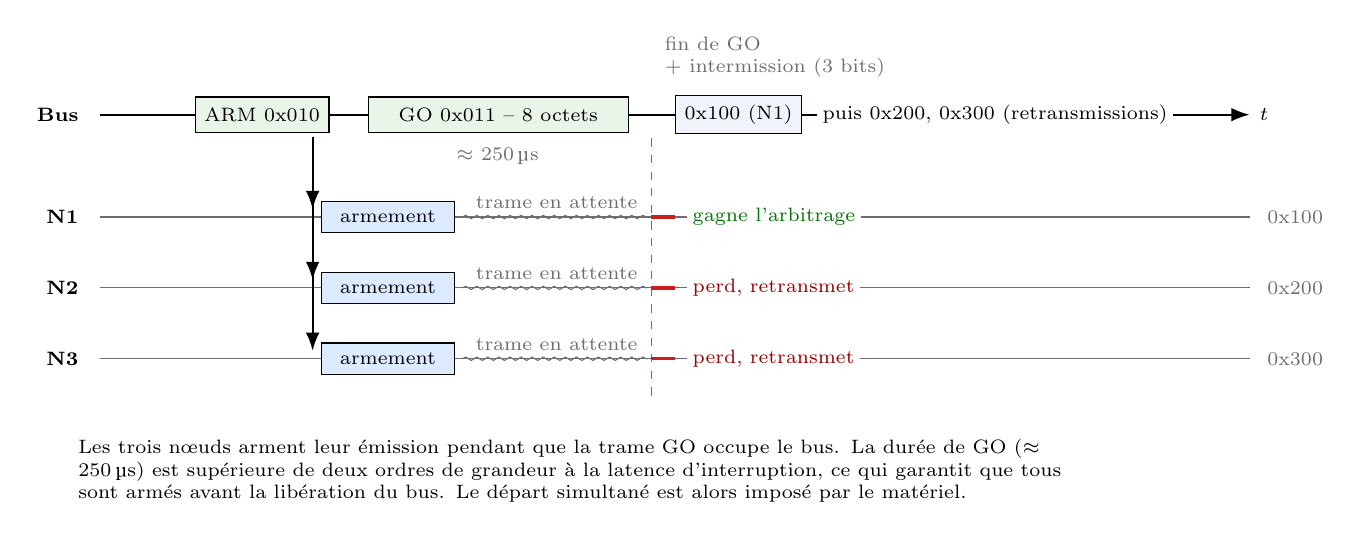
\begin{tikzpicture}[x=1cm,y=1cm]

\def\rowBus{0}      % ligne bus
\def\rowA{-1.3}   % N1
\def\rowB{-2.2}   % N2
\def\rowC{-3.1}   % N3

% ---- axe temps ----
\draw[-{Latex}, thick] (0,\rowBus) -- (14.6,\rowBus) node[right, font=\scriptsize] {$t$};
\node[font=\scriptsize\bfseries, anchor=east] at (-0.15,\rowBus) {Bus};

% ---- trames sur le bus ----
\node[draw, fill=toolfill, minimum width=1.5cm, minimum height=0.45cm, anchor=west,
      font=\scriptsize] (ARM) at (1.2,\rowBus) {ARM 0x010};
\node[draw, fill=toolfill, minimum width=3.3cm, minimum height=0.45cm, anchor=west,
      font=\scriptsize, inner sep=2pt] (GO) at (3.4,\rowBus) {GO 0x011 -- 8 octets};
\node[font=\scriptsize, text=grey, anchor=north] at (5.05,\rowBus-0.3) {$\approx$ \SI{250}{\micro s}};
\draw[dashed, grey] (7.0,\rowBus-0.3) -- (7.0,\rowC-0.55);
\node[font=\scriptsize, text=grey, anchor=south west, align=left] at (7.05,\rowBus+0.35)
  {fin de GO\\ + intermission (3 bits)};
\node[draw, fill=nodefill, minimum width=1.6cm, minimum height=0.45cm, anchor=west,
      font=\scriptsize] (WIN) at (7.3,\rowBus) {0x100 (N1)};
\node[font=\scriptsize, fill=white, inner sep=2pt, anchor=west] at (9.1,\rowBus)
  {puis 0x200, 0x300 (retransmissions)};

% ---- lignes des noeuds ----
\foreach \yy/\nom/\id in {\rowA/N1/0x100, \rowB/N2/0x200, \rowC/N3/0x300}
{
  \draw[grey] (0,\yy) -- (14.6,\yy);
  \node[font=\scriptsize\bfseries, anchor=east] at (-0.15,\yy) {\nom};
  \node[font=\scriptsize, text=grey, anchor=west] at (14.7,\yy) {\id};
  % armement a la reception de ARM
  \draw[-{Latex}, thick] (2.7,\rowBus-0.28) -- (2.7,\yy+0.1);
  \node[draw, fill=mcufill, minimum width=1.7cm, minimum height=0.4cm, anchor=west,
        font=\scriptsize] at (2.8,\yy) {armement};
  % attente
  \draw[decorate, decoration={snake, amplitude=0.6pt, segment length=4pt}, grey]
    (4.6,\yy) -- (6.95,\yy);
  \node[font=\scriptsize, text=grey, anchor=south, fill=white, inner sep=1pt] at (5.8,\yy+0.06) {trame en attente};
  % emission simultanee
  \draw[very thick, canh] (7.0,\yy) -- (7.3,\yy);
}
% resultat de l'arbitrage
\node[font=\scriptsize, anchor=west, text=green!45!black, fill=white, inner sep=2pt] at (7.45,\rowA) {gagne l'arbitrage};
\node[font=\scriptsize, anchor=west, text=red!60!black, fill=white, inner sep=2pt]   at (7.45,\rowB) {perd, retransmet};
\node[font=\scriptsize, anchor=west, text=red!60!black, fill=white, inner sep=2pt]   at (7.45,\rowC) {perd, retransmet};

\node[font=\scriptsize, anchor=north west, text width=13cm, align=left] at (-0.4,\rowC-0.9)
  {Les trois nœuds arment leur émission pendant que la trame GO occupe le bus. La durée de GO
   ($\approx$ \SI{250}{\micro s}) est supérieure de deux ordres de grandeur à la latence
   d'interruption, ce qui garantit que tous sont armés avant la libération du bus. Le départ
   simultané est alors imposé par le matériel.};

\end{tikzpicture}
\caption{Protocole ARM/GO : la trame GO sert de fenêtre d'occupation du bus, pendant laquelle
les contendants arment leur émission. L'arbitrage qui suit est donc réel.}
\label{fig:armgo}
\end{figure}

\begin{table}[H]
\centering\small
\begin{tabular}{llp{8.4cm}}
\toprule
\textbf{Identifiant} & \textbf{Nom} & \textbf{Rôle} \\
\midrule
0x010 & ARM & Ordre d'armement. À sa réception, chaque contendant place sa trame de test dans
sa boîte d'émission et incrémente son compteur \emph{ARM reçus}. \\
0x011 & GO & Trame de \num{8} octets sans contenu utile : elle occupe le bus le temps que tous
les contendants aient armé. \\
\bottomrule
\end{tabular}
\caption{Identifiants de service à réserver. Ces deux identifiants doivent être déclarés comme
réservés dans les ICD, faute de quoi un groupe partenaire pourrait les réutiliser pour un
signal applicatif.}
\end{table}

\paragraph{Contrôle de validité du test.} Si un nœud arme trop tard (interruption masquée,
traitement bloquant), il rate la fenêtre et émet seul juste après : il apparaîtrait alors
comme vainqueur sans avoir affronté personne, et le résultat serait faux sans que rien ne le
signale. La parade est le compteur \emph{ARM reçus} affiché sur chaque écran : avant de lire
le classement, on vérifie que tous les contendants affichent la même valeur. En cas d'écart,
le test est invalide et doit être rejoué.

\paragraph{Résultat attendu.} Après \num{1000} cycles, les afficheurs doivent montrer un
classement conforme à l'ordre des identifiants, l'identifiant le plus faible étant le plus
prioritaire :

\begin{table}[H]
\centering\small
\begin{tabular}{llrrr}
\toprule
\textbf{Nœud} & \textbf{Identifiant} & \textbf{Gagnés} & \textbf{Perdus} & \textbf{ARM reçus} \\
\midrule
N1 & 0x100 & \num{1000} & \num{0} & \num{1000} \\
N2 & 0x200 & \num{0} & \num{1000} & \num{1000} \\
N3 & 0x300 & \num{0} & \num{1000} & \num{1000} \\
\bottomrule
\end{tabular}
\caption{Résultat attendu du test d'arbitrage. Tout écart sur la colonne \emph{ARM reçus}
invalide le test.}
\end{table}

\paragraph{Réutilisabilité.} Le protocole ARM/GO n'utilise que des trames CAN standard et
aucun signal hors bus. Il constitue donc une brique que les groupes partenaires peuvent
reprendre telle quelle pour vérifier l'arbitrage sur leur propre réseau.

% =====================================================================
\section{Tableau de câblage}
% =====================================================================
\todo{tableau exhaustif broche à broche pour les cinq connecteurs et le boîtier de fautes}

% =====================================================================
\section{Configuration logicielle minimale}
% =====================================================================
\todo{paramètres FDCAN pour \SI{500}{kbit/s} en mode Classic (horloge, prescaler, segments), broches, bibliothèque HAL}

% =====================================================================
\section{Protocole de validation}
\label{sec:protocole}
% =====================================================================
\todo{sept tests au format objectif / montage / procédure / critère de réussite / résultat}

% =====================================================================
\section{Historique des versions}
% =====================================================================
\begin{table}[H]
\centering\small
\begin{tabular}{llp{9cm}}
\toprule
\textbf{Version} & \textbf{Date} & \textbf{Modifications} \\
\midrule
v0.1 & \docdate & Création. Architecture de principe et schémas électriques (\S2, \S4).
Autres sections en squelette. \\
\bottomrule
\end{tabular}
\end{table}

\end{document}